\documentclass[12pt,a4paper,notitlepage]{article}
\usepackage[utf8]{inputenc}
\usepackage[a4paper,textwidth=17cm, top=2cm, bottom=3.5cm]{geometry}
\usepackage[T1]{fontenc}
\usepackage[
    backend=biber,
    style=numeric,
    natbib=true,
    url=true, 
    doi=true,
    eprint=false
    ]{biblatex}
\addbibresource{directions.bib}
\usepackage{amssymb,amsmath}
\usepackage{listings}
\usepackage{eurosym}
\usepackage{wasysym}
\usepackage{amsthm}
\usepackage{tabularx}
\usepackage{multirow}
\usepackage{multicol}
\usepackage{tikz}
\usepackage{hyperref}
\usepackage{tabularx}
\usepackage{commath}
\usepackage{graphicx,color}
\usepackage{subcaption}
\usepackage{float}
\usepackage{footmisc}
\usepackage{array}
\usepackage[underline=false]{pgf-umlsd}
\usetikzlibrary{calc}
%\usepackage[pdftex]{graphicx,color}
%\usepackage{epstopdf}

\newcommand{\foonote}[1]{\footnote{#1}}
\newcommand{\degree}{\ensuremath{^\circ}}
\newcolumntype{P}[1]{>{\centering\arraybackslash}p{#1}}

\author{Sebastian Götte {\texttt<secureusb@jaseg.net>} @Mori lab, Waseda University}
\title{Research directions in secure USB devices}
\date{November 19 2018}
\begin{document}
\maketitle

\section{Problem definition}
A computer's USB interface is hard to secure. Though overall security is quite good today, the USB interface has not
received enough attention. In particular HIDs are a problem, as they are naturally very highly privileged.
Off-the-shelf USB HID attack tools exist. In particular from a security point of view extremely bad ideas such as
WebUSB\cite{misc01} are set to increase this already large attack surface even further.

\section{State of the art}
Research exists in various directions.
\begin{itemize}
    \item USB firewalls have been proposed\cite{tian01,angel01,kang01,bates01,loe01}.
    \item USB device authentication has been proposed\cite{usb01,griscioli01,wang01,he01}.
    \item USB bus encryption has been proposed\cite{neugschwandtner01,weinstein01}.
    \item For wireless protocols, every conceivable pairing model has been tried. However, not many have been applied to
        USB\cite{arun01,uzun01,kobsa01,saxena01}.
    \item Compartmentalized systems such as QubesOS have been implemented
\end{itemize}

\begin{table}
    \setlength{\extrarowheight}{5pt}
    \begin{tabular}{l|P{10mm}|P{15mm}|P{15mm}|P{15mm}|P{17mm}|P{25mm}|}
                                &\multicolumn{3}{c|}{\bfseries Attacks}                                             & \multicolumn{2}{c|}{\bfseries Eavesdropping} & \multirow{2}{25mm}{\centering\bfseries Backwards\newline compatible} \\\cline{2-6}
                                & \bfseries HID     &\bfseries Host\newline exploit &\bfseries Device\newline exploit&\bfseries Bus-level &\bfseries Physical layer    & \\\hline
        Firewalls               & $\bigcirc$        & $\triangle$                   & $\times$                      & $\triangle$   & $\times$          & $\bigcirc$ \\
        Device authentication   & $\bigcirc$        & $\times$                      & $\times$                      & $\triangle$   & $\times$          & $\times$ \\
        Bus encryption          & $\triangle$       & $\times$                      & $\times$                      & $\bigcirc$    & $\bigcirc$        & $\times$ \\
        Plain QubesOS setup\footnotemark 
                                & $\triangle$       & $\triangle$                   & $\triangle$                   & $\triangle$   & $\times$          & $\bigcirc$ \\
        Our work                & $\bigcirc$        & $\bigcirc$                    & $\bigcirc$                    & $\bigcirc$    & $\bigcirc$        & $\bigcirc$
    \end{tabular}
    \caption{Comparison of approaches to USB security}
    \label{approach_comparison}
\end{table}
\footnotetext{Requires separate USB host controller for HIDs}

Overall, QubesOS is the only significant practical advance towards securing this interface. Other approaches have not
been successful so far. A likely reason for this is large market inertia and necessary backwards-compatibility.

QubesOS approaches the problem by running a separate VM with the USB host controllers mapped through via IOMMU. This VM
runs a linux kernel with a small set of white-listed USB device drivers (HID and mass storage device) and a USB-over-IP
backend. A set of Qubes services pass through any HID input arriving inside this VM into dom0, and coordinate exporting
USB mass storage devices as Xen block devices. Any other USB devices can be passed-through to other VMs through
USB-over-IP-over-QubesRPC, a Xen vChan-based inter-VM communication system.

QubesOS is still lacking in that it's compartmentalization becomes essentially useless when it is used with a USB HID
keyboard that does not have its own dedicated PCIe USB host controller, as any normal desktop and most recent laptop
computers. The issue here is that USB HID is neither authenticated nor encrypted, and the untrusted USB VM sits in the
middle of this data stream, which thus allows it trivial privilege escalation.

\section{Project goal}
The goal of SecureHID is to enable the first reasonably secure system using both HID and arbitrary untrusted devices on
the same USB host controller, based on QubesOS. SecureHID consists of a USB HID encryption box to be put between
keyboard and computer and a piece of software run inside QubesOS. After initial pairing with the host software, the
encryption box will encrypt and sign any USB HID input arriving from the keyboard and forward the encrypted data to the
host. The host software running outside the untrusted USB VM will receive the encrypted and signed data from the
untrusted USB VM, verify and decrypt it, and inject the received HID input events into Qubes's input event handling
system.

\subsection{Audio and other sensitive USB devices}
This system is sufficient to secure any USB setup, especially unmodified desktop PCs or laptops where a USB host
controller is shared between both HIDs and other devices. Attack surface is reduced such that a \emph{full compromise}
of the system becomes unlikely, since plain HID is no longer supported. The remaining attack surface consists only of a
\emph{compromise of the USB VM}. This attack surface is small enough that other sensitive devices such as USB audio
devices can safely be connected. A compromise of the USB driver VM no longer gives full system access, but at best
allows listening in on the microphone. Since a compromised USB VM does not have network access, such an attack will be
mostly harmless in most scenarios. Additionally, the most likely attacking devices would be custom hardware or a
smartphone. Custom hardware can easily be outfitted with a microphone, essentially turning it into a bug irrespective of
USB functionality, and smartphones already have microphones by definition.

A practical mitigation to this issue would be to simply connect microphones either to a PCIe-based sound card as in most
laptops, or to simply unplug the microphone when not used.

\subsection{USB physical-level and bus-level attacks}
Since sensitive HIDs are isolated from other USB devices effectively on a separate bus, bus-level attacks such as
\textcite{neugschwandtner01} are entirely prevented. Even much scarier physical attacks on USB such as \textcite{su01}
are prevented given an adequate hardware implementation, which fortunately is no too complicated.

\subsection{Diagram of a conventional setup}
\begin{figure}[H]
    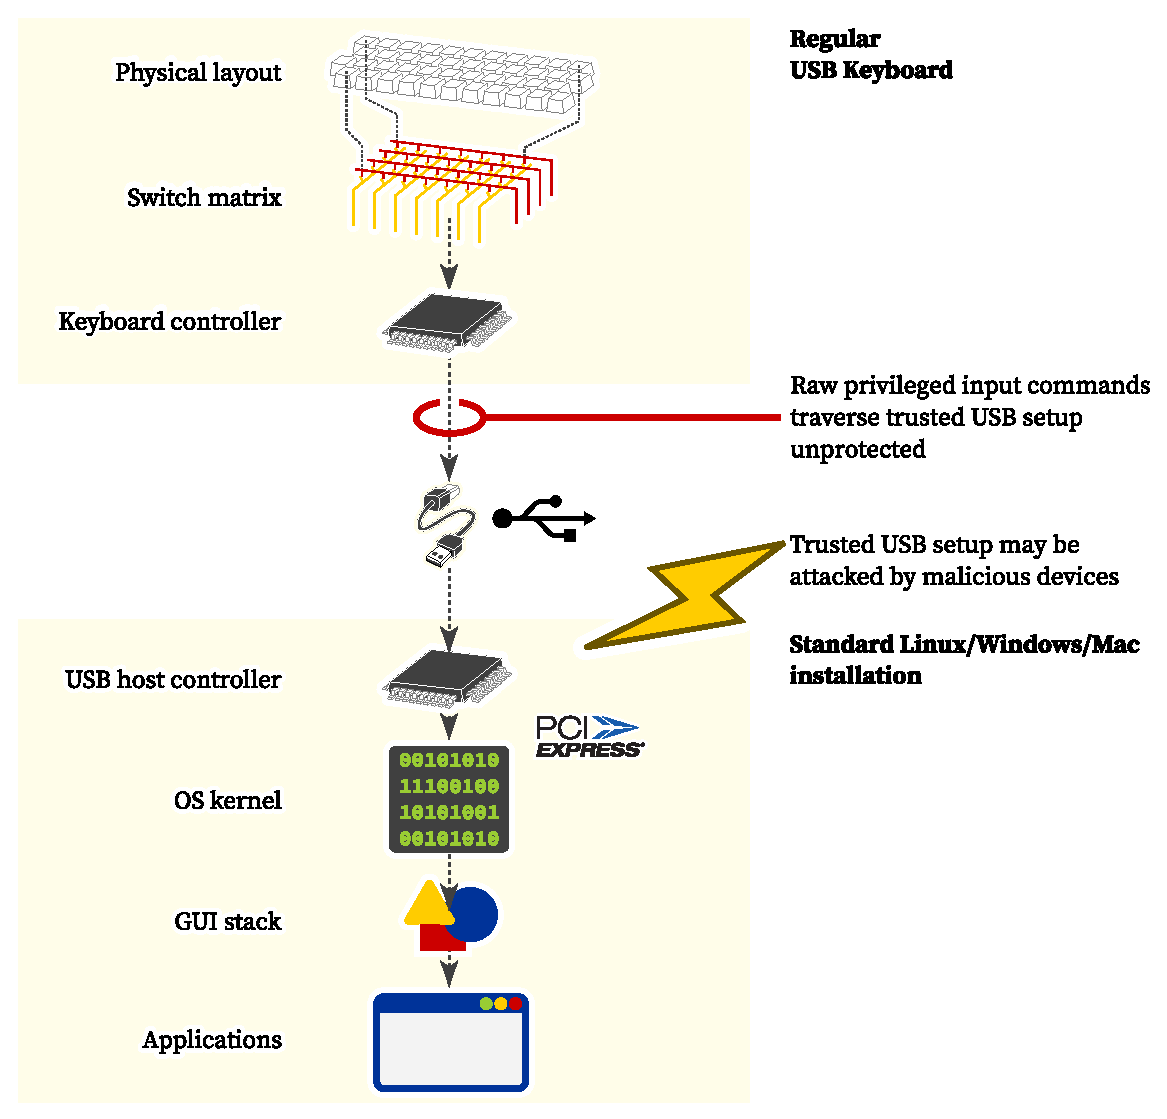
\includegraphics[scale=0.8]{system_diagram_without_secureusb.eps}
    \caption{Diagram of a conventional unprotected system}
    \label{diagram_without}
\end{figure}
\subsection{Diagram of a SecureHID-protected system}
\begin{figure}[H]
    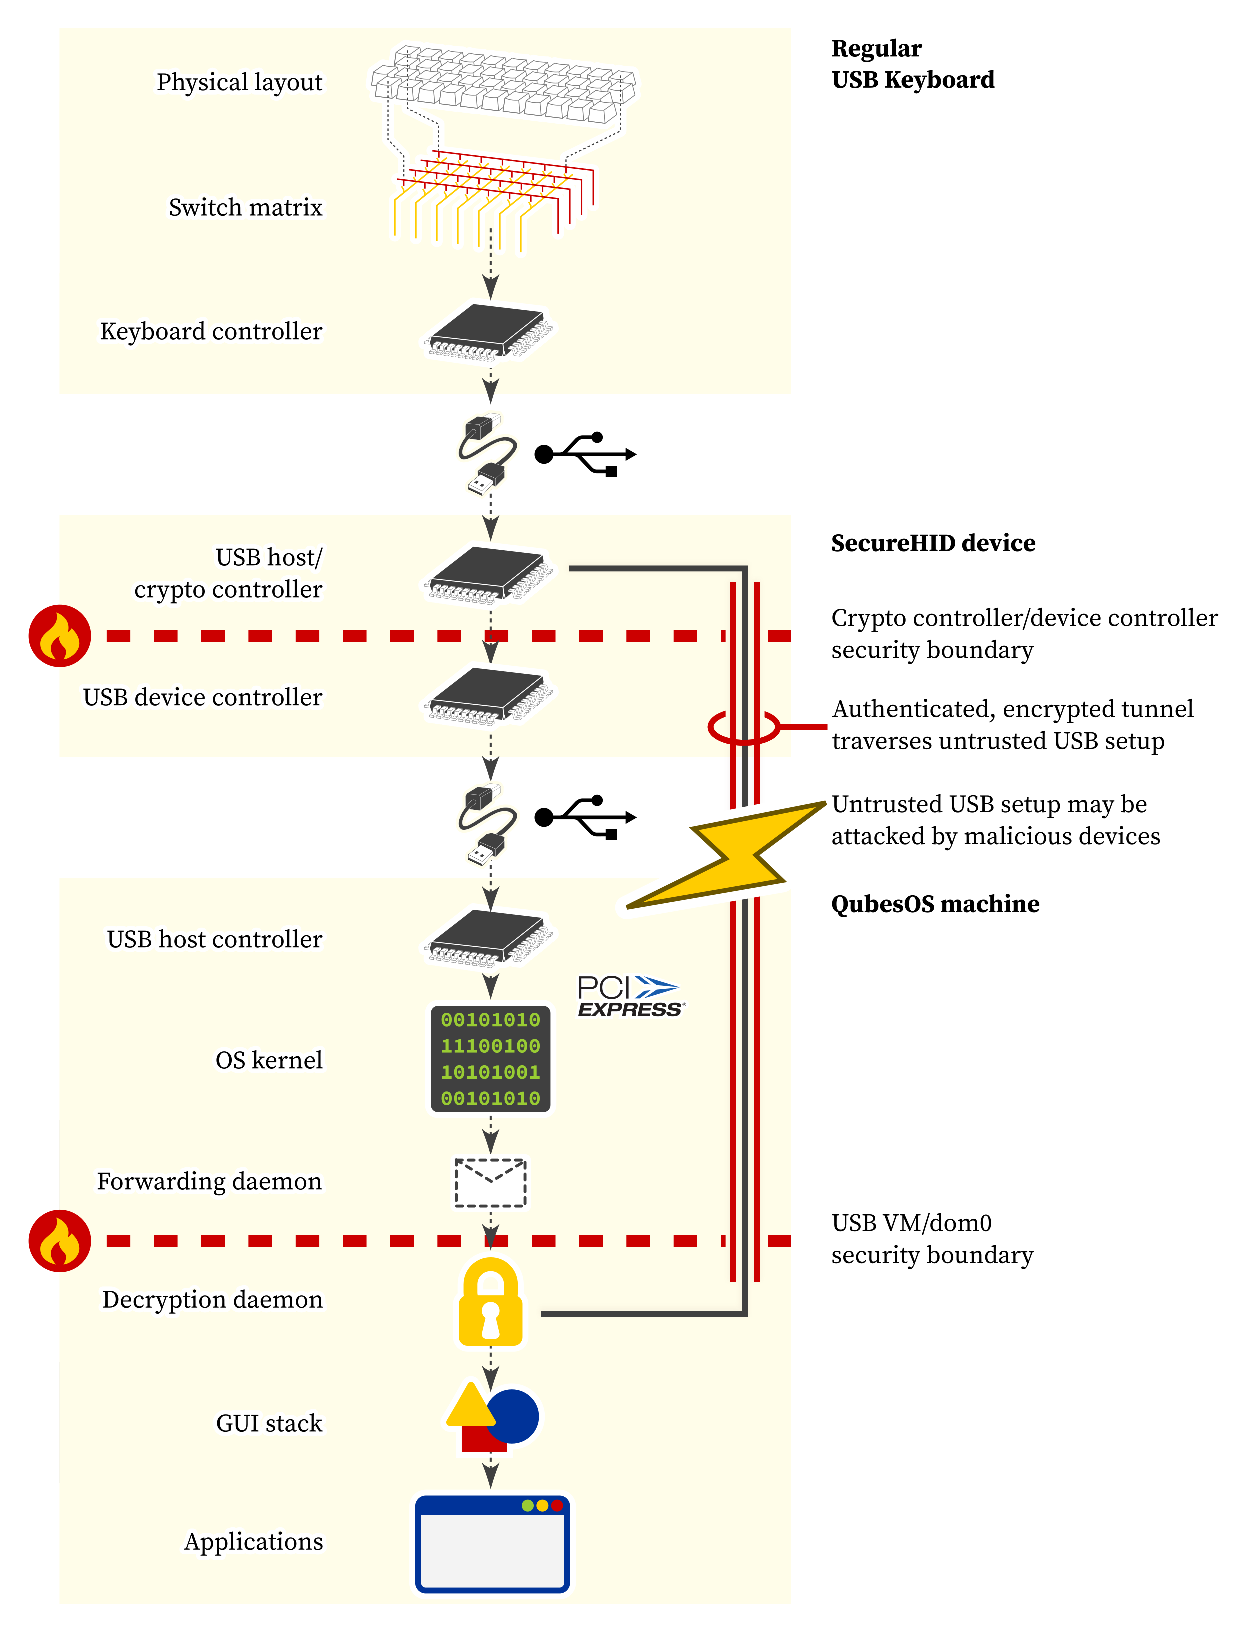
\includegraphics[scale=0.8]{system_diagram_with_secureusb.eps}
    \caption{Diagram of a SecureHID-protected system}
    \label{diagram_with}
\end{figure}

\subsection{Key points}
\begin{itemize}
    \item A practical example of a complete, secure USB system using Qubes
    \item A novel interactive user-friendly side channel-based cryptographic handshaking scheme
    \item An example of a secure USB-based protocol
\end{itemize}

\section{Project state}
A working prototype has been completed.

\subsection{Completed}
\begin{itemize}
    \item Rough protocol design
    \item Protocol implementation based on \textcite{perrin01} using noise-c (microcontroller) and noiseprotocol (python/host)
    \item SRAM-based key storage with SRAM wear prevention
    \item host/device signature checking
    \item host/device key generation
    \item proper circuit design because I was bored last weekend (see appendix \ref{ch:renderings})
\end{itemize}

\subsection{Open issues}
\begin{itemize}
    \item Both noise-c and noiseprotocol have poor code and API quality. Since most noise functionality is not needed,
        just implement the protocol in bare C/python based on cryptographic primitives and scrap higher-level protocol
        implementations (though they've been useful so far during prototyping).
    \item Implement HID mouse host support
    \item Test USB hub support
    \item Replace the serial link with a custom USB link using an STM32F103 instead of the CH340G USB/serial converter
    \item Properly integrate prototype host client with qubes infrastructure
    \item Implement photodiode/monitor-based pairing side-channel
\end{itemize}

\section{Possible directions}
\begin{itemize}
    \item Elaborate handshake security properties
        \begin{itemize}
            \item Possibly investigate other applications of this type of interactive handshake
            \item Possibly contrast to carmera/other backchannel systems
            \item IMHO the pairing scheme is the most interesting part of this project from a scientific point of view
        \end{itemize}
    \item Elaborate overall security properties of QubesOS-based system
    \item Elaborate possible DisplayPort/HDMI-based display encryption
    \item Elaborate possible encrypted remote input (SSH) setups
        \begin{itemize}
            \item This might turn out to be really interesting
            \item For this to be usable the host needs to tell the device at least which keyslot to use which could turn
                out to be complex to implement securely
            \item Considering complexity, this might turn into its own research project
        \end{itemize}
    \item Create custom hardware prototype
    \item Showcase secure hardware interface design, contrast with wireguard protocol design
        \begin{itemize}
            \item Formally derive handshake security properties
            \item Formally derive host/device protocol security properties using noise spec
            \item Formally verify and thouroughly unit-test the host/device protocol implementation on all layers
            \item IMHO this is the most interesting part of this project from an engineering point of view
        \end{itemize}
    \item Benchmark cryptography routines (will likely turn out to be ``wayyy fast'' for HID, fast enough for full-speed
        USB. High-speed cannot be done with the current architecture as we can't get data out the chip at high-speed
        data rates. \textcite{srivaths01} raise the issue of running crypto on embedded systems, but in this case it
        turns out with somewhat modern hardware and cryptography there is no problem at all.
\end{itemize}

\newpage
\appendix
\section{High-level protocol design}

\begin{figure}
    \centering
    \begin{sequencediagram}
        \newinst{kbd}{Keyboard}
        \newinst[3]{dev}{SecureHID}
        \newinst[5]{host}{Host}

        \mess{host}{}{dev}
        \path (mess from) -- (mess to) node[midway, above] {\emph{COBS sync (null byte)}};
        \mess{host}{}{dev}
        \draw[->,>=angle 60] (mess from) -- (mess to) node[midway, above] {\textsc{Initiate Handshake}};

        \begin{sdblock}{Noise XX handshake}{}
            \mess{host}{}{dev}
            \path (mess from) -- (mess to) node[midway, above] {$\textsc{Handshake}, e$};
            \mess{dev}{}{host}
            \path (mess from) -- (mess to) node[midway, above] {$\textsc{Handshake}, e,ee,s,es$};
            \mess{host}{}{dev}
            \path (mess from) -- (mess to) node[midway, above] {$\textsc{Handshake}, s,se$};
        \end{sdblock}

        \begin{sdblock}{Pairing}{Triggered by user interaction after unsuccessful handshake}
            \mess{dev}{}{host}
            \draw[->,>=angle 60] (mess from) -- (mess to) node[midway, above] {\textsc{Pairing Start}};
            \stepcounter{seqlevel}

            \mess{kbd}{keystroke}{dev}
            \addtocounter{seqlevel}{-1}
            \mess{dev}{}{host}
            \path (mess from) -- (mess to) node[midway, above] {$\textsc{Pairing Input},E(\text{keystroke})$};
            \stepcounter{seqlevel}
            \mess{kbd}{}{dev}
            \addtocounter{seqlevel}{-1}
            \path (mess from) -- (mess to) node[midway, above] {keystroke};
            \path (mess from) -- (mess to) node[midway, above, yshift=5mm] {$\vdots$};
            \mess{dev}{}{host}
            \path (mess from) -- (mess to) node[midway, above] {$\textsc{Pairing Input},E(\text{keystroke})$};
            \path (mess from) -- (mess to) node[midway, above, yshift=5mm] {$\vdots$};
            \stepcounter{seqlevel}

            \mess{kbd}{}{dev}
            \addtocounter{seqlevel}{-1}
            \path (mess from) -- (mess to) node[midway, above] {\emph{enter}};
            \mess{dev}{}{host}
            \draw[->,>=angle 60] (mess from) -- (mess to) node[midway, above] {\textsc{Pairing Success}};
        \end{sdblock}

        \begin{sdblock}{Input passthrough}{Started after successful handshake or pairing}
            \mess{kbd}{keystroke}{dev}
            \path (mess from) -- (mess to) node[midway, below, yshift=-2mm] {$\vdots$};

            \addtocounter{seqlevel}{-1}
            \mess{dev}{}{host}
            \path (mess from) -- (mess to) node[midway, above] {$\textsc{Data},E(\text{keystroke})$};
            \path (mess from) -- (mess to) node[midway, below, yshift=-2mm] {$\vdots$};
            \stepcounter{seqlevel}
        \end{sdblock}
    \end{sequencediagram}
    \caption{A successful prototype protocol pairing}
    \label{protocol_diagram}
\end{figure}

The basic protocol consists of two stages: \textsc{pairing} and \textsc{data}. When the device powers up, it enters
\textsc{pairing} state. When the host enumerates a new device, it enters \textsc{pairing} state. If any fatal
communication errors occur, both host and device re-enter \textsc{pairing} state. To make the implementation robust
against host software crashing, devices being unplugged etc. without opening it up to attacks, the host can request the
device to re-enter \textsc{pairing} state a limited number of times after powerup.

\textsc{pairing} state consists of a number of substates as set by \textcite{perrin01}. The device runs noise's
\textsc{XX} scheme, i.e. both host and device each contribute both one ephemeral key $e$ and one static key $s$ to the
handshake, and the public halves of the static keys are transmitted during handshake encrypted by the emphemeral keys.
This scheme provides forward-secrecy without MITM protection.

The cryptographic primitives instantiated in the prototype are X25519 for the ECDH primitive, BLAKE2s as a hash and
ChaCha20-Poly1305 as AEAD for the data phase. ECDH instead of traditional DH was chosen for its small key size and fast
computation. Since no variant of RSA is used, key generation is fast. An ad-hoc prototype device-side random number
generator has been implemented based on BLAKE2s and the STM32's internal hardware RNG.

A successful protocol run always starts like this:
\begin{enumerate}
\item \textbf{Handshake.} \textsc{device} is connected to \textsc{host}
\item \textsc{host} initiates pairing by sending \textsc{initiate handshake} to device
\item \textsc{device} and \textsc{host} follow noise state machine for \textsc{XX} handshake
\item After the handshake completes, both \textsc{device} and \textsc{host} have received each other's static public key
    $rs$ and established a shared secret connection key. At this point, the possibility of an MITM attacker having
    actively intercepted the handshake remains.
\item \textbf{Channel binding.} Both \textsc{device} and \textsc{host} calculate the \emph{handshake hash} as per noise spec\cite{perrin01}. This
    hash uniquely identifies this session and depends on both local and remote ephemeral and static keys $le, re, ls,
    rs$.  Both parties encode a 64-bit part of this hash into a sequence of english words by dictionary lookup. This
    sequence of words is called the \emph{fingerprint} of the connection.
\item \textsc{host} prompts the user to enter the \emph{fingerprint} into a keyboard connected to \textsc{device}.
\item As the user enters the \emph{fingerprint}, \textsc{device} relays any input over the yet-unauthenticated encrypted
    noise channel to \textsc{host}. \textsc{host} displays the received user input in plain text in a regular input
    field in the pairing GUI. This display is only for user convenience and not relevant to the cryptographic handshake.
    A consequence of this is that a MITM could observe the \emph{fingerprint}\footnote{
        A MITM could also modify the fingerprint information sent from \textsc{device} to \textsc{host}. This would be
        very obvious to the user, since the fingerprint appearing on the \textsc{host} screen would differ from what she
        types.
    }.
\item When the user has completed entering the fingerprint, the device checks the calculated fingerprint against the
    entered data. If both match, the host is signalled \textsc{success} and \textsc{data} phase is entered. If they do
    not match, the host is signalled \textsc{failure}\footnote{
        Note that this means a MITM could intercept the \textsc{failure} message and forge a \textsc{success} message.
        This means both are just for user convenience \emph{absent} an attacker. If an attacker is present, she will be
        caught in the next pairing step.
    } and \textsc{pairing} state is re-entered unless the maximum number of tries since powerup has been exceeded.
    Failure is indicated to the user by \textsc{device} through a very annoying beep accompanied by angrily flashing
    LEDs.
\item \textbf{Data phase.} \textsc{host} asks the user for confirmation of pairing \emph{in case the device did not sound an alarm} by
    pressing a button on the GUI. When the user does this, the host enters \textsc{data} state and starts input
    passthrough.
\end{enumerate}

Roughly speaking, this protocol is secure given that the only way to MITM a (EC)DH key exchange is to perform two (EC)DH key exchanges with both parties, then relay messages. Since both parties have different static keys, the resulting two (EC)DH sessions will have different handshake hashes under the noise framework. The channel binding step reliably detects this condition through an out-of-band transmission of the \textsc{host} handshake hash to \textsc{device}.

The only specialty here is that this OOB transmission is relayed back from \textsc{device} to \textsc{host} allowing the MITM to intercept it. This is only done for user convenience absent a MITM and the result is discarded by \textsc{host}. Since the handshake hash does as a hash does not leak any sensitive information about the keys used during the handshake, it being exposed does not impact protocol security.

\section{PCB design renderings}
\label{ch:renderings}

\begin{figure}[H]
    \centering
    \begin{subfigure}[b]{0.8\textwidth}
        \centering
        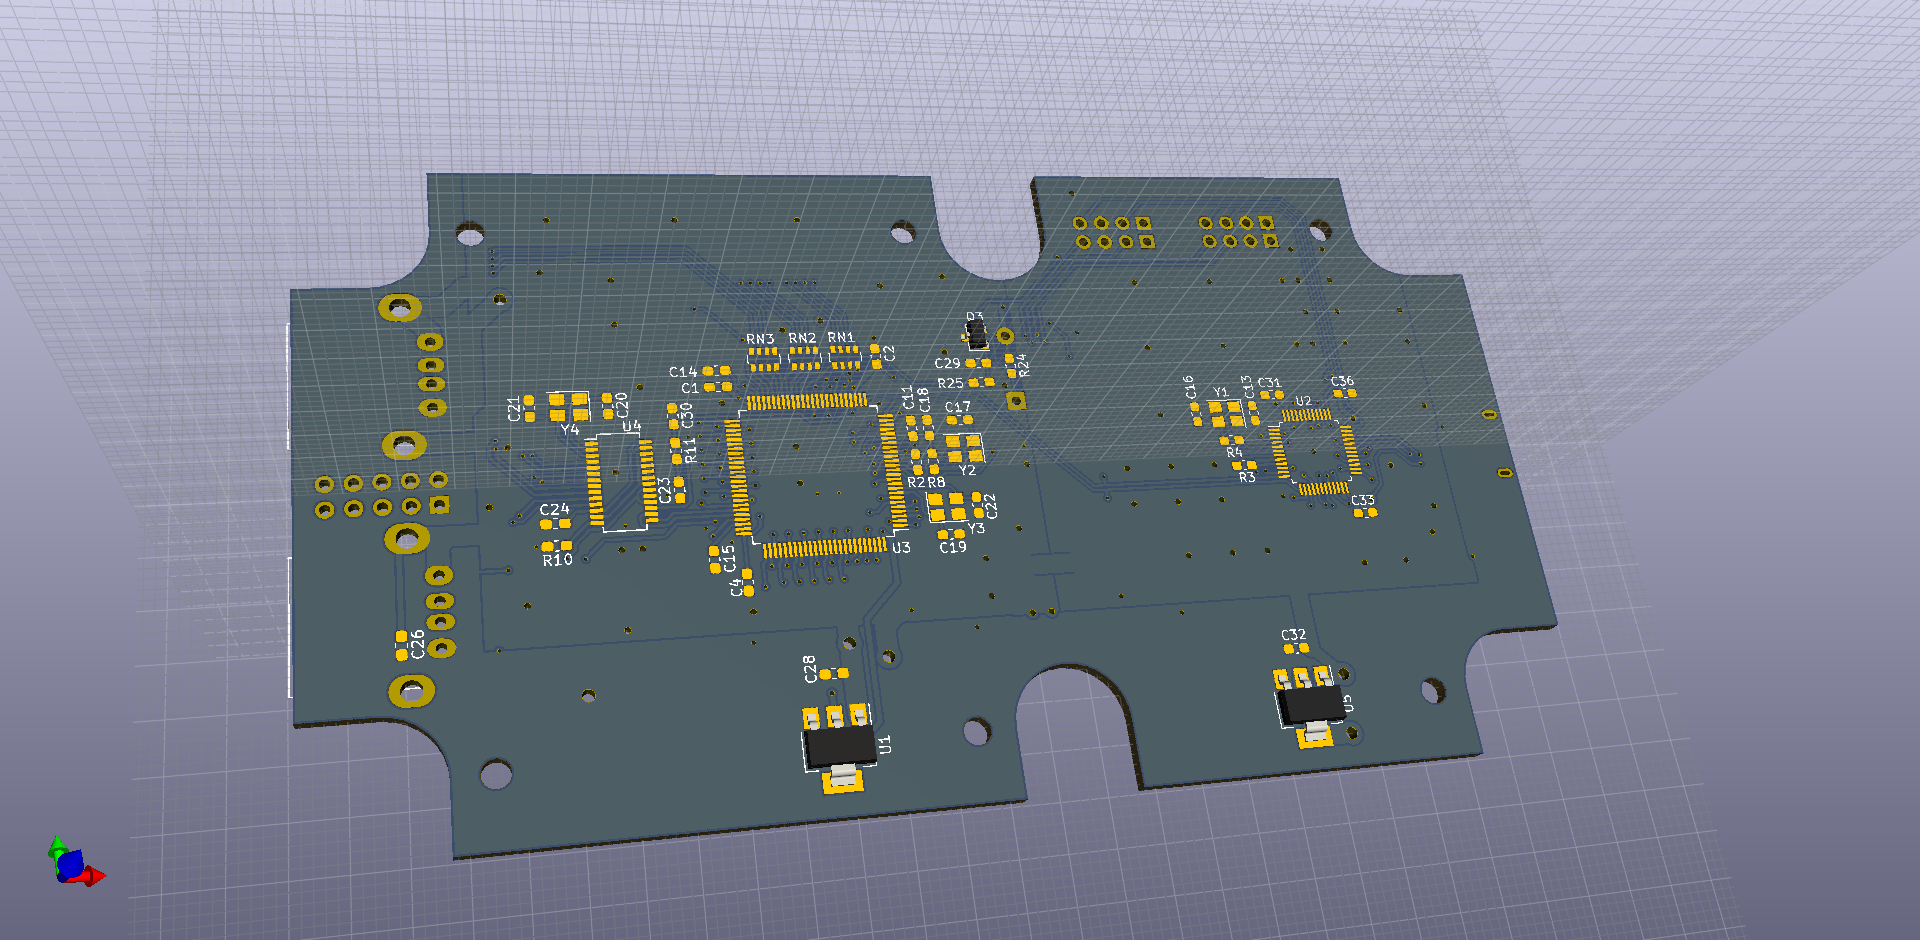
\includegraphics[width=0.8\textwidth]{pcb_front.png}
        \caption{PCB front}
    \end{subfigure} %
    \begin{subfigure}[b]{0.8\textwidth}
        \centering
        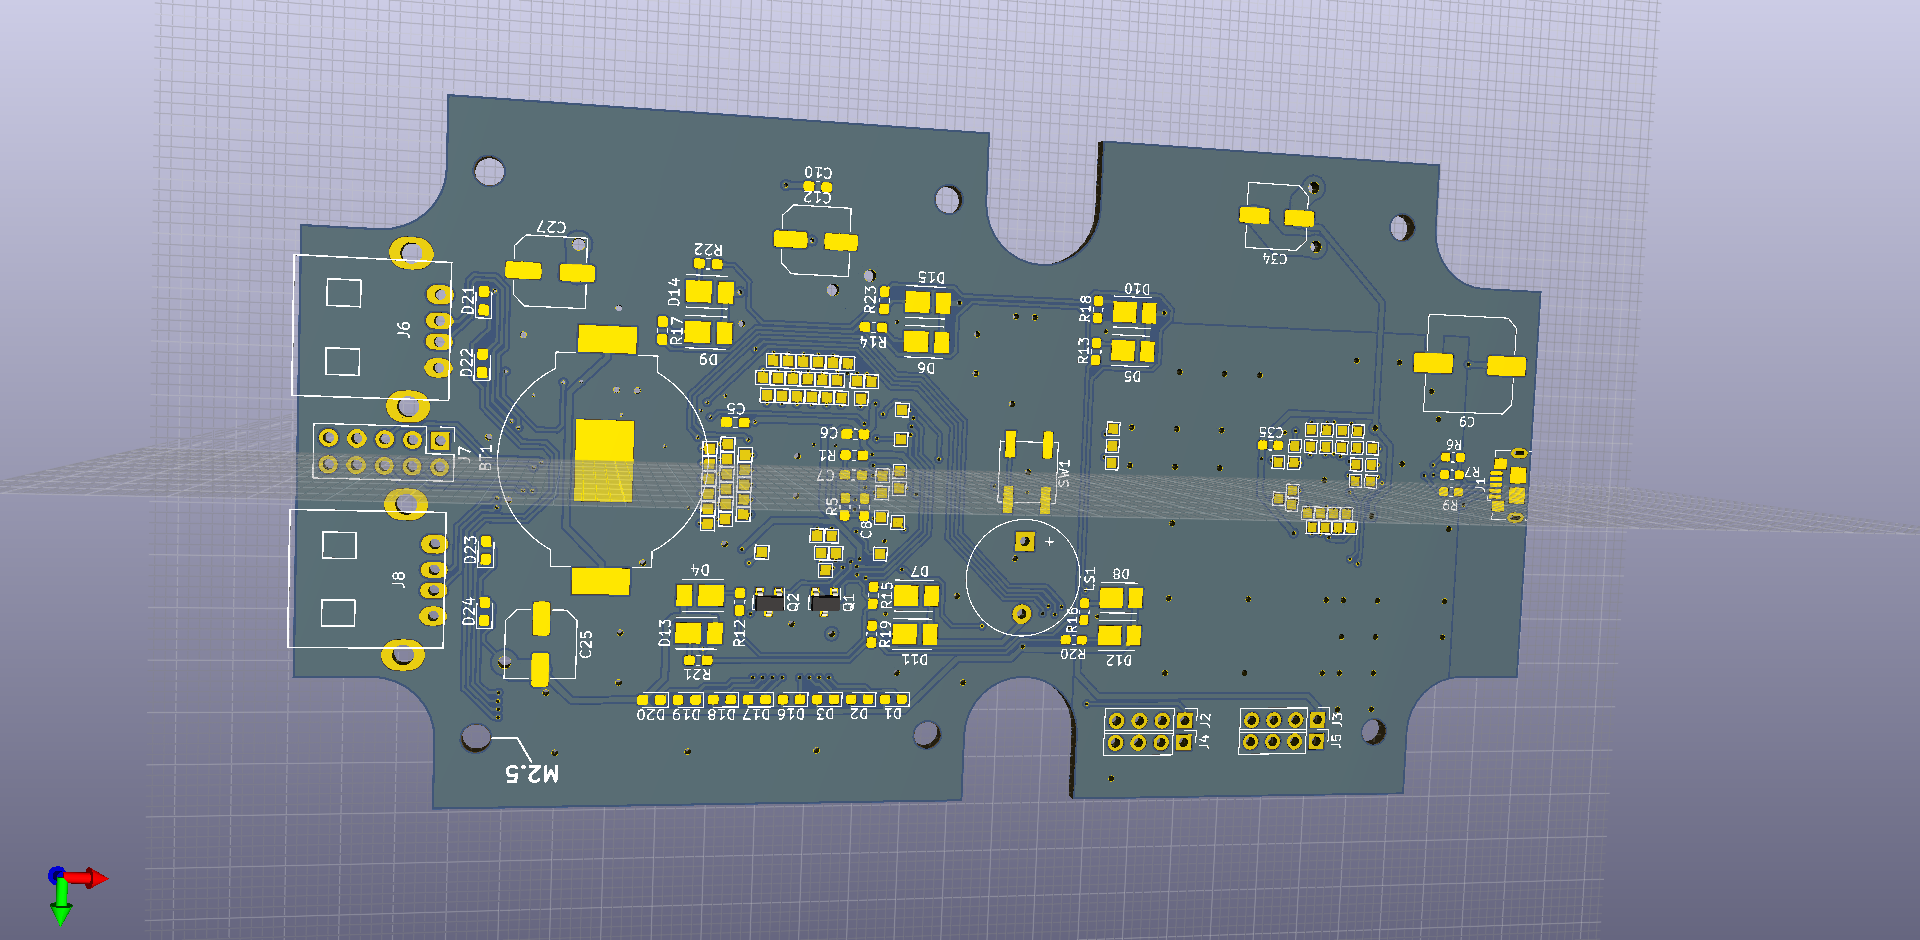
\includegraphics[width=0.8\textwidth]{pcb_back.png}
        \caption{PCB back}
    \end{subfigure}
    \caption{PCB design 3D renderings}
    \label{fig:pcb3d}
\end{figure}

\begin{figure}[H]
    \centering
    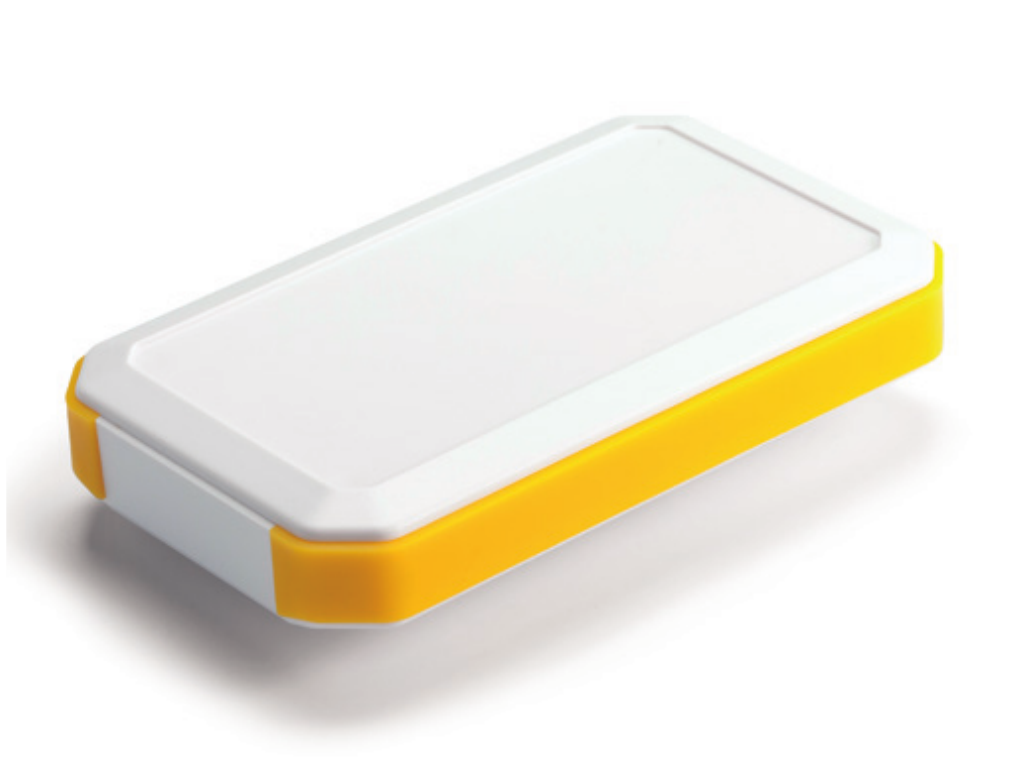
\includegraphics[width=0.6\textwidth]{takachi_case.png}
    \caption{Off-the-shelf enclosure the PCB is made to fit}
    \label{fig:case}
\end{figure}

%\subsection{Attack surface in reasonably secure systems}
%\begin{figure}
%\tikzstyle{block} = [rectangle, draw, text centered, minimum height=4em]
%\begin{tikzpicture}[node distance=2cm, auto]
%   \node[block](matrix){Key matrix}
%   \node[block](hidctrl){Keyboard controller}
%   \node[block](hubs){USB hubs}
%   \node[block](roothub){USB host controller}
%   \node[block](pcie){PCIe bus}
%   \node[block](sys-usb-kernel){USB VM kernel}
%   \node[block](sys-usb-agent){USB VM userspace agent}
%   \node[block](dom0){dom0 agent}
%\end{tikzpicture}
%\label{qubes-hid-stack}
%\caption{The USB HID input stack in a QubesOS setup}
%\end{figure}

\nocite{*}
\printbibliography

\end{document}
